\section{Gate-Treiber}\label{Appendix:TMC6200}

\subsection{Standard-Schaltkreis}\label{Appendix:Schaltung_TMC6200}

\begin{figure}[H]
	\centering
	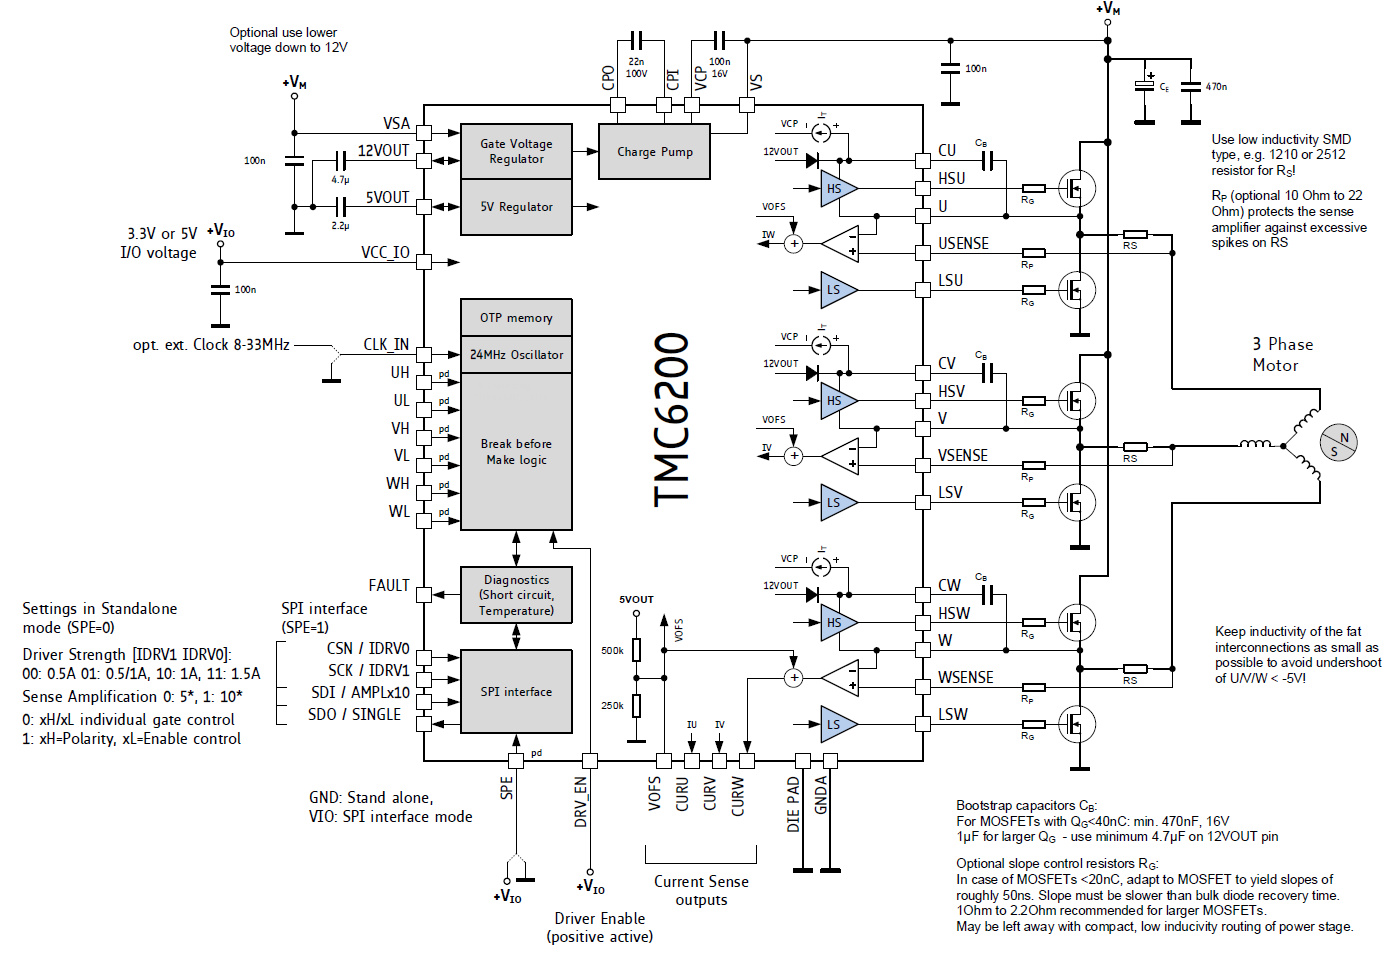
\includegraphics[width=0.8\textwidth]{graphics/Standard_Application_Cirquit_TMC6200.png}
	\caption{Standard-Anwendungs-Schaltung Gate-Treiber.\cite[S.1]{trinamicmotion_control_gmbh__co_kg_tmc6200_2019}}
	\label{fig:Schaltung_TMC6200}
\end{figure}

\subsection{Blockdiagramm}\label{Appendix:Blockdiagramm_TMC6200}

\begin{figure}[H]
	\centering
	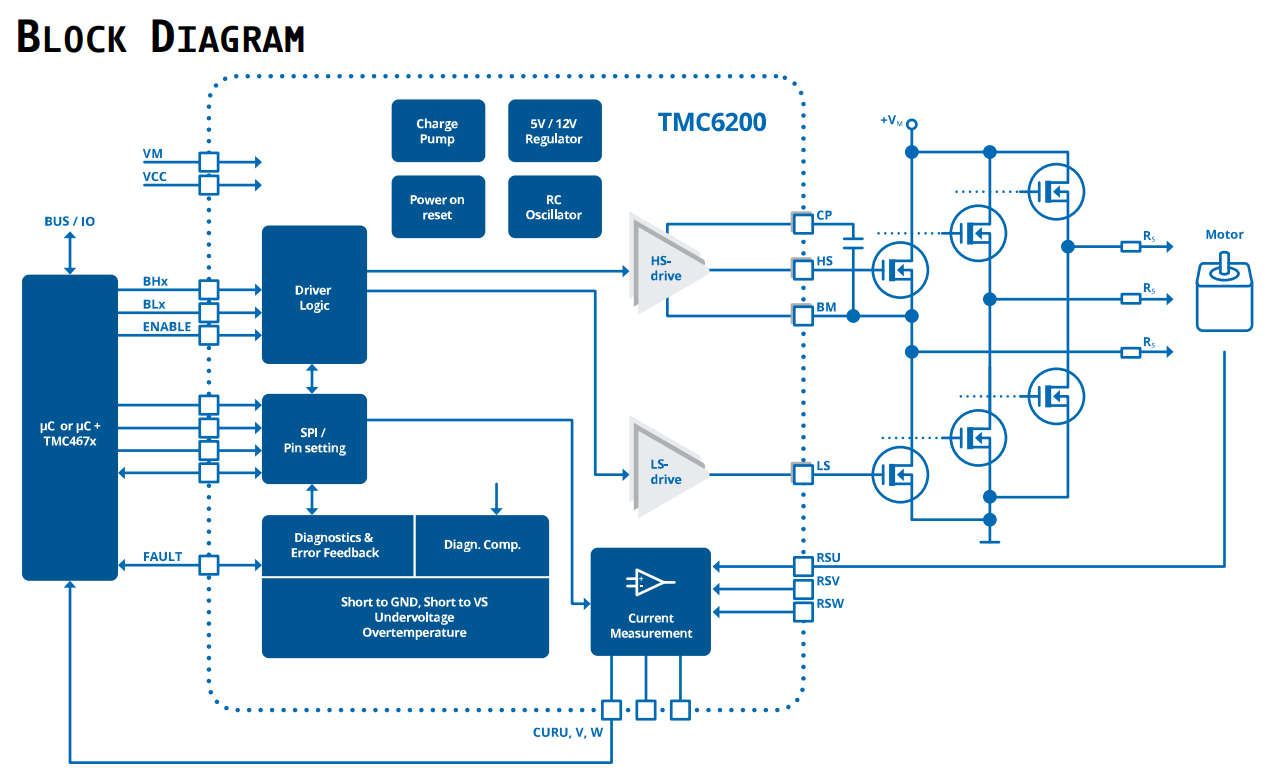
\includegraphics[width=0.8\textwidth]{graphics/Blockdiagramm_TMC6200.png}
	\caption{Blockdiagramm Gate-Treiber.\cite[S.5]{trinamicmotion_control_gmbh__co_kg_tmc6200_2019}}
	\label{fig:Blockdiagramm_TMC6200}
\end{figure}

%\subsection{Externe Gate-Spannungsversorgung}\label{Appendix:Gate_Spannungsversorgung}
%
%\begin{figure}[H]
%	\centering
%	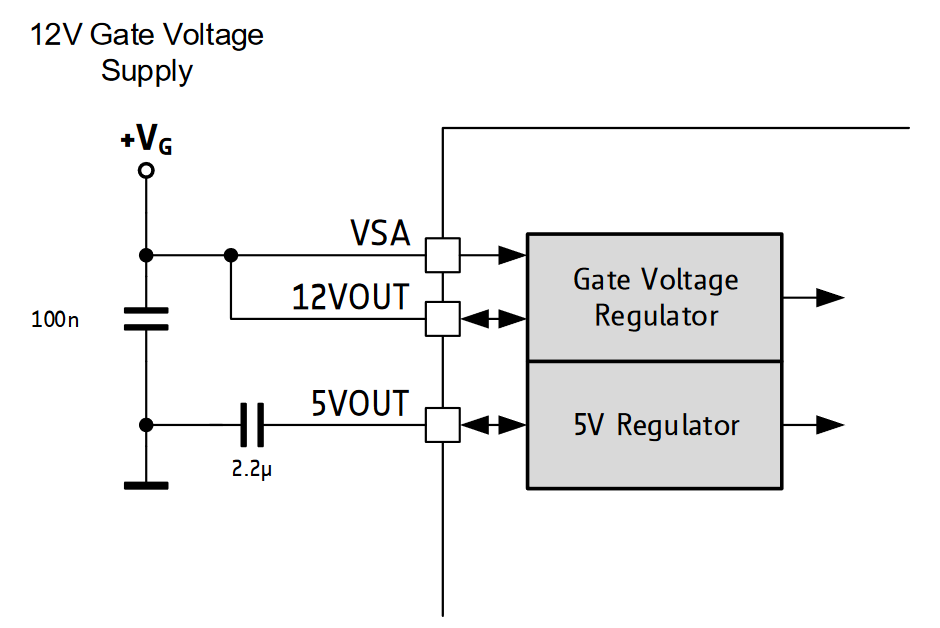
\includegraphics[width=0.4\textwidth]{graphics/Schema_Gate_Treiber_Gatespannung}
%	\caption{Schema externe Gate-Spannungsversorgung.\cite[S.11]{trinamicmotion_control_gmbh__co_kg_tmc6200_2019}}
%	\label{fig:Schema_Gate_Treiber_Gatespannung}
%\end{figure}

%\subsection{Inbetriebnahme}
%\subsubsection{Inbetriebnahme Setup}\label{Appendix:TMC6200_Setup}

%\begin{figure}[H]
%	\centering
%	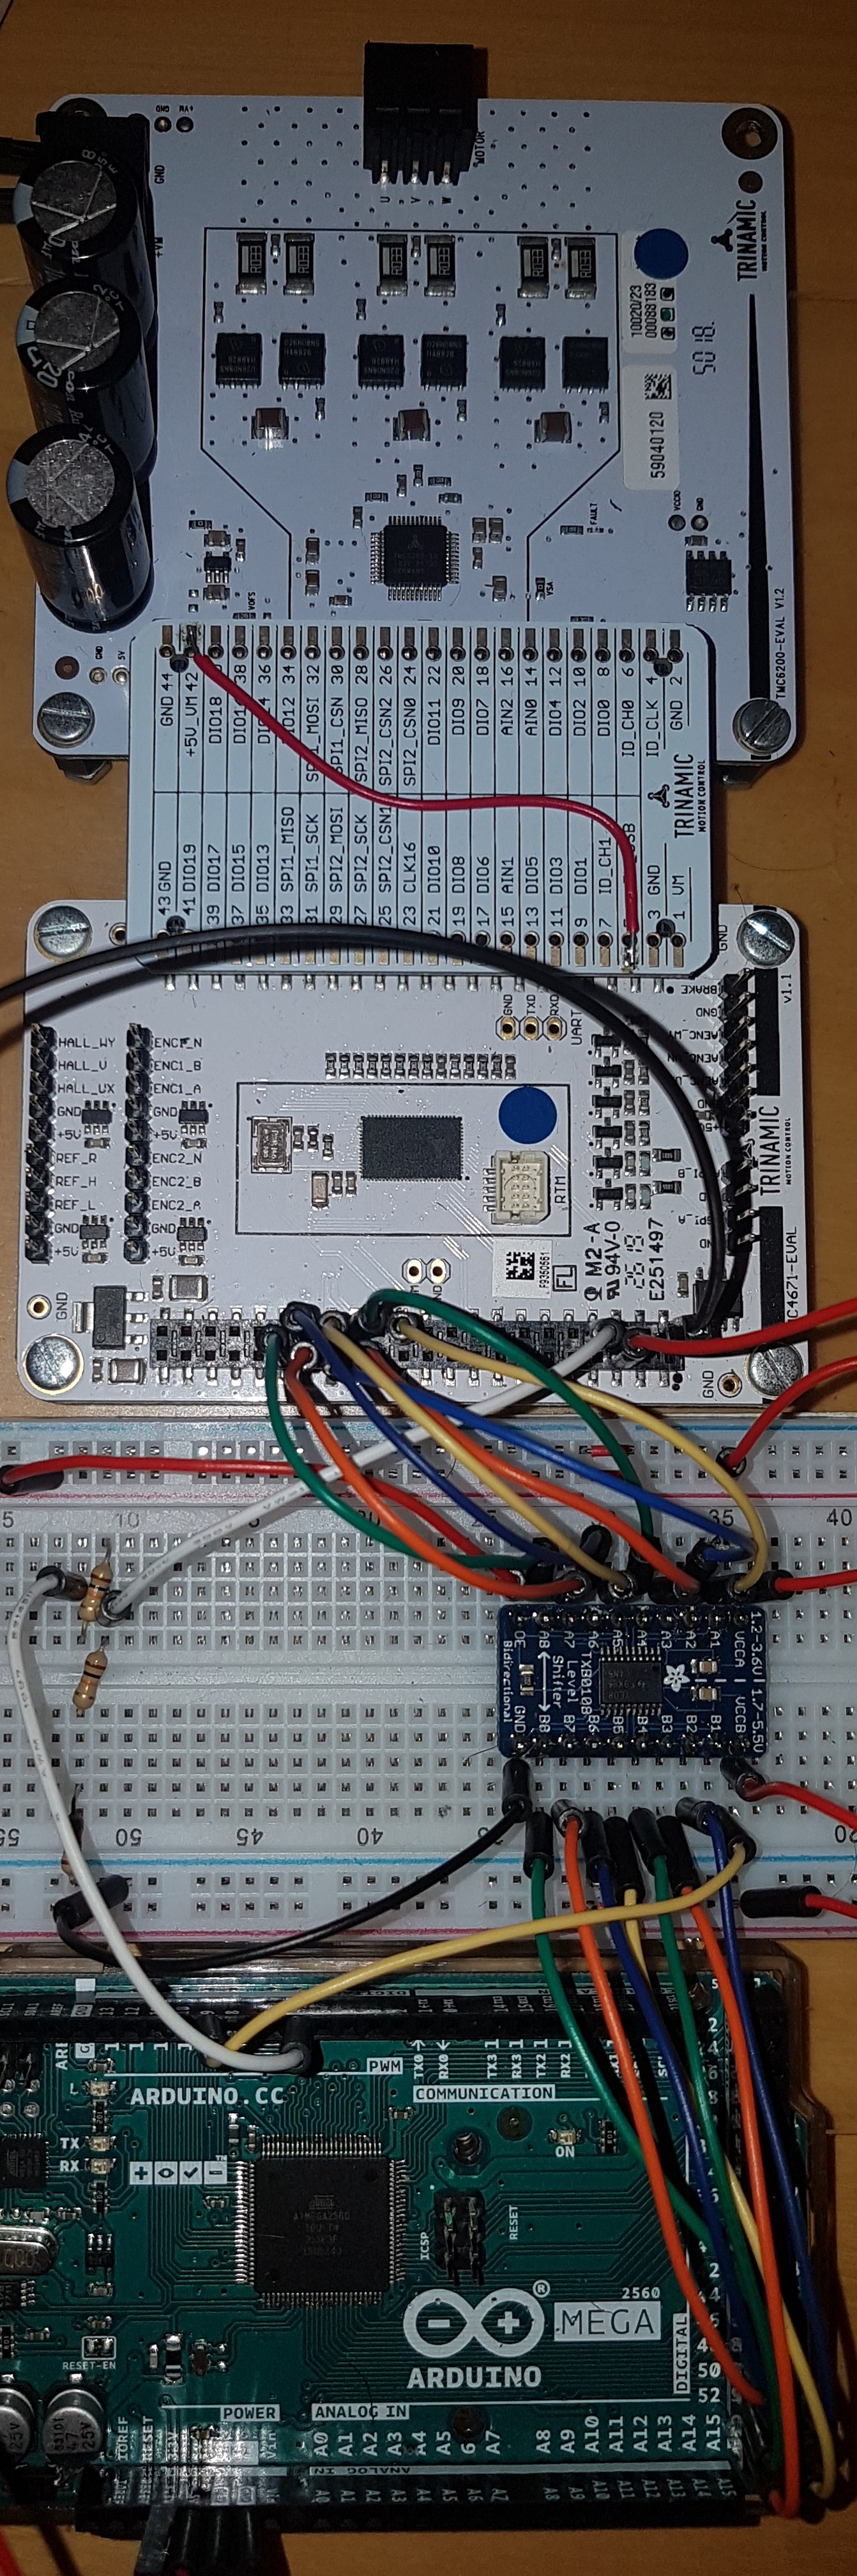
\includegraphics[angle=270,width=\textwidth]{graphics/2_komplett1}
%	\caption{Gesamtansicht Setup.}
%	\label{fig:2_komplett1}
%\end{figure}

%\begin{figure}[H]
%	\centering
%	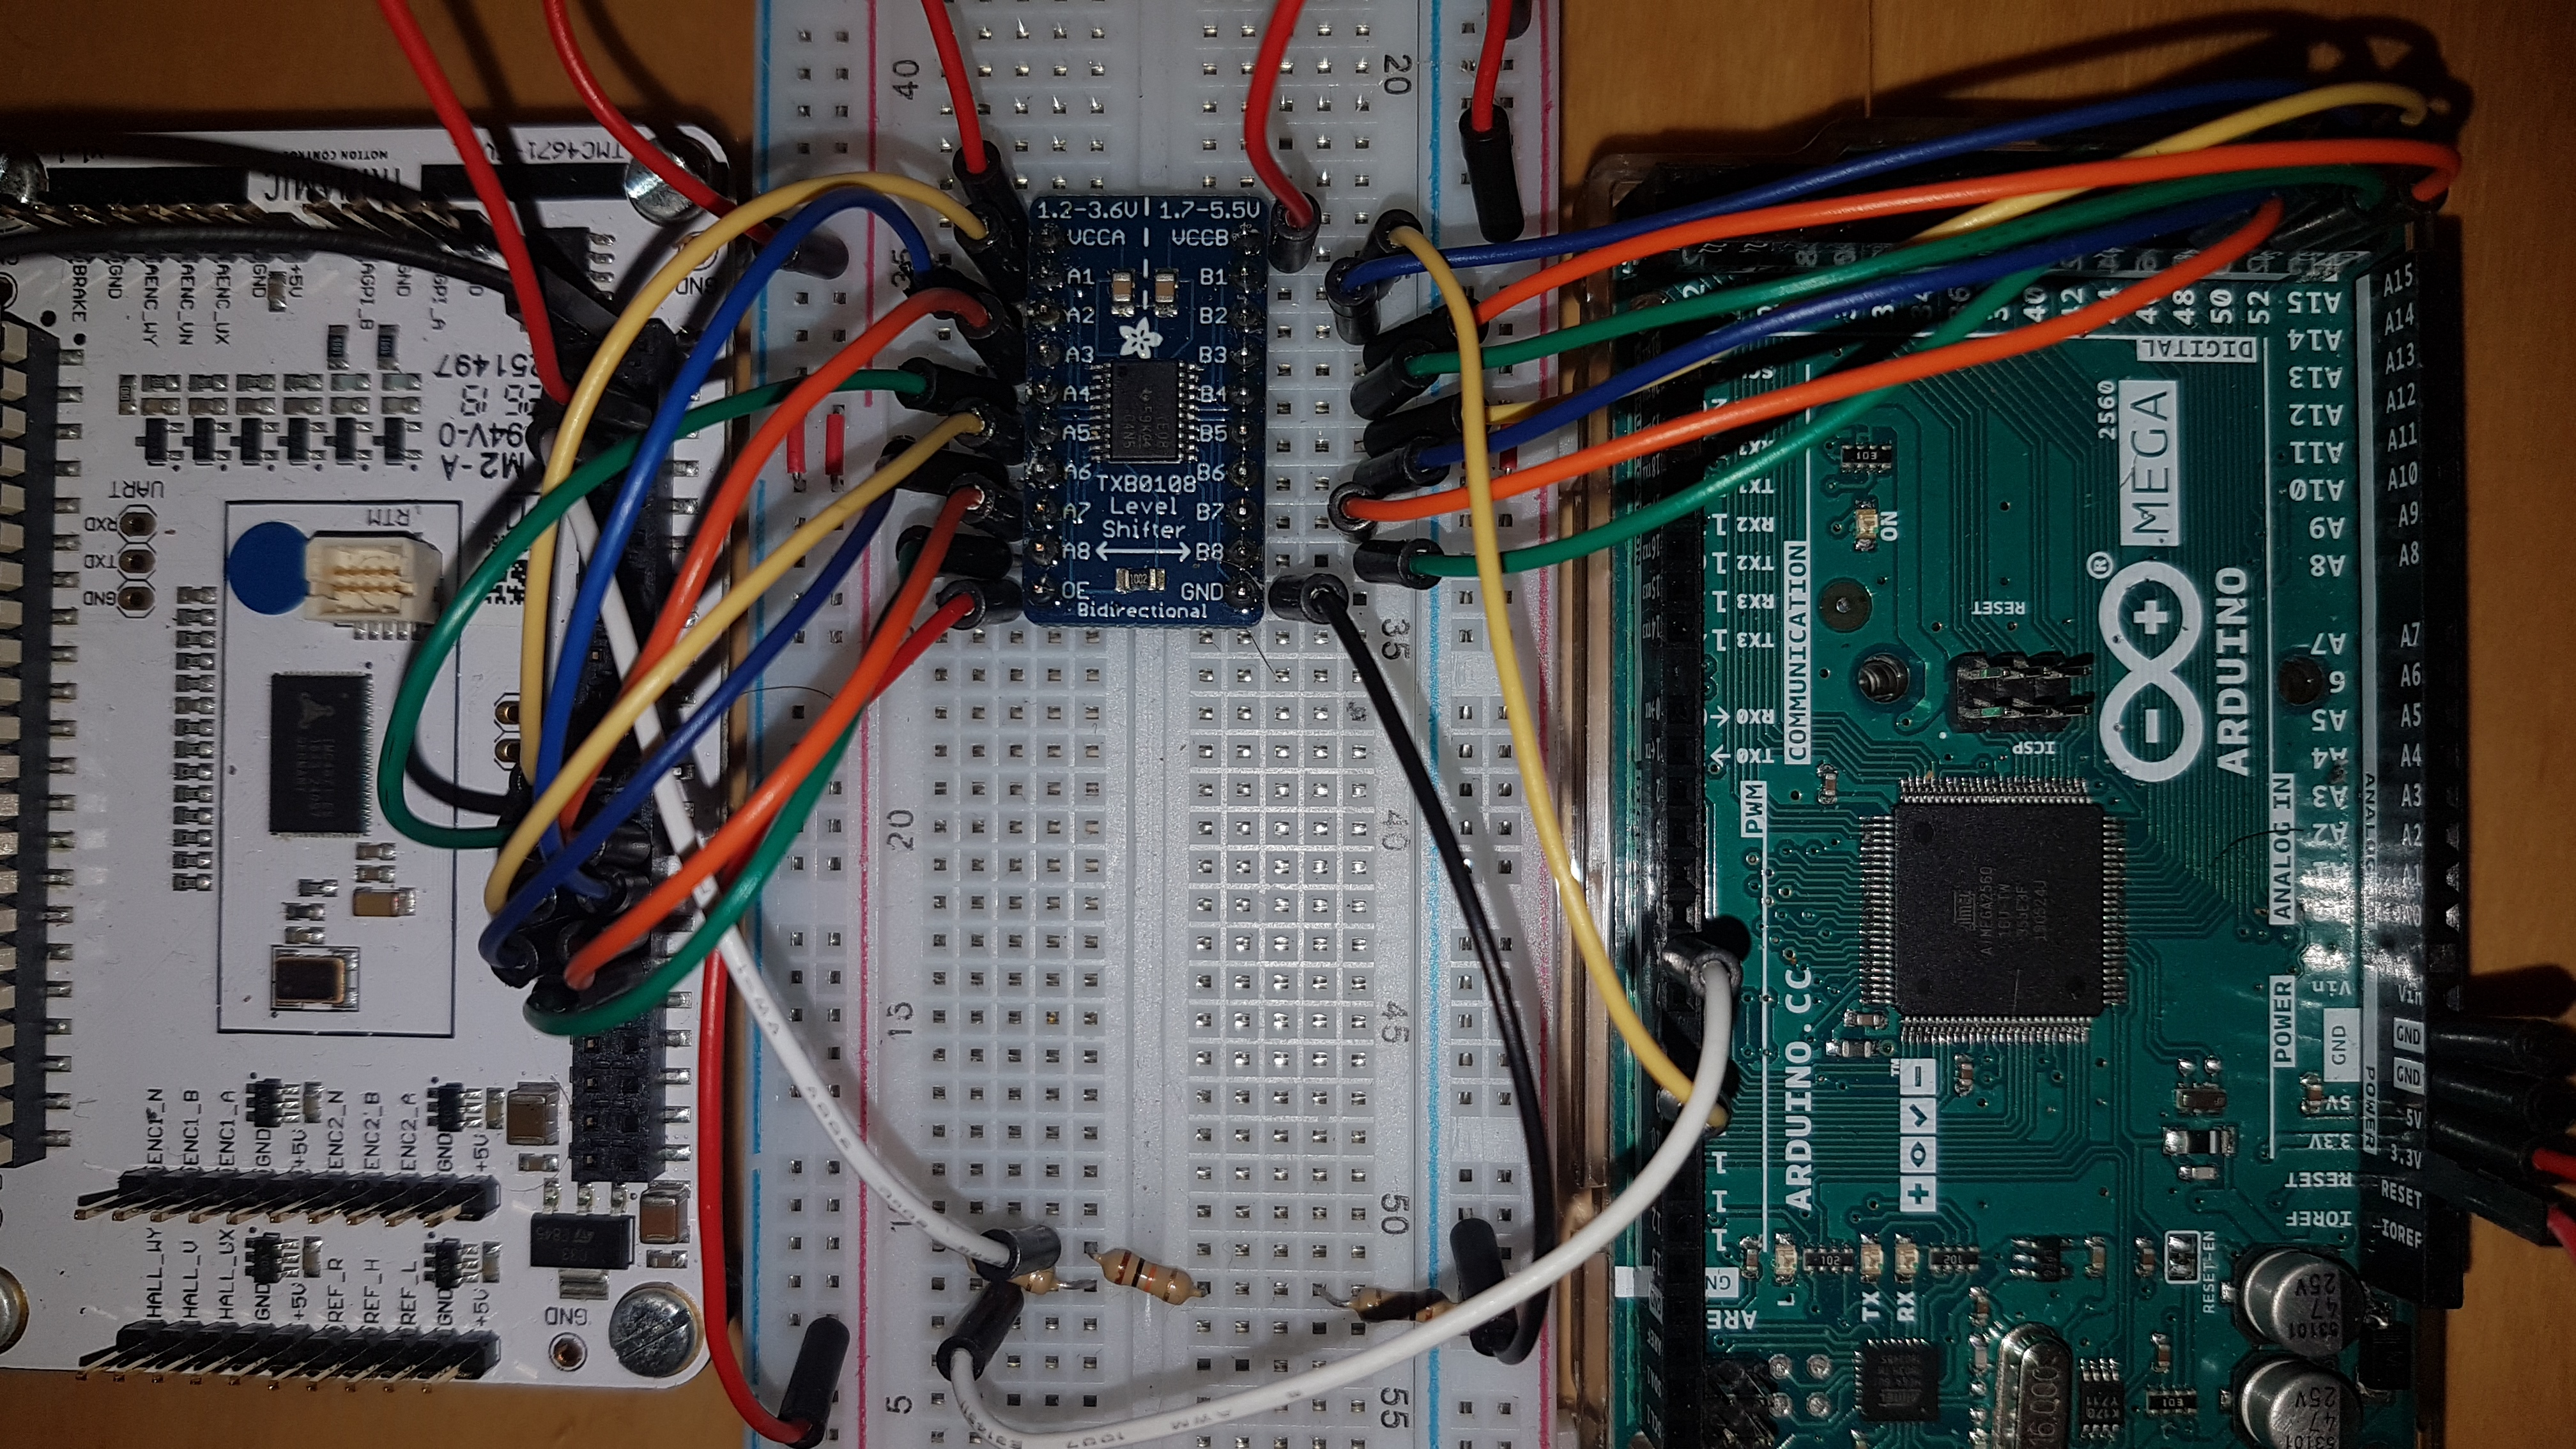
\includegraphics[angle=180,width=\textwidth]{graphics/2_komplett2}
%	\caption{Gesamtansicht Setup Wiring.}
%	\label{fig:1_komplett}
%\end{figure}
%
%\begin{figure}[H]
%	\centering
%	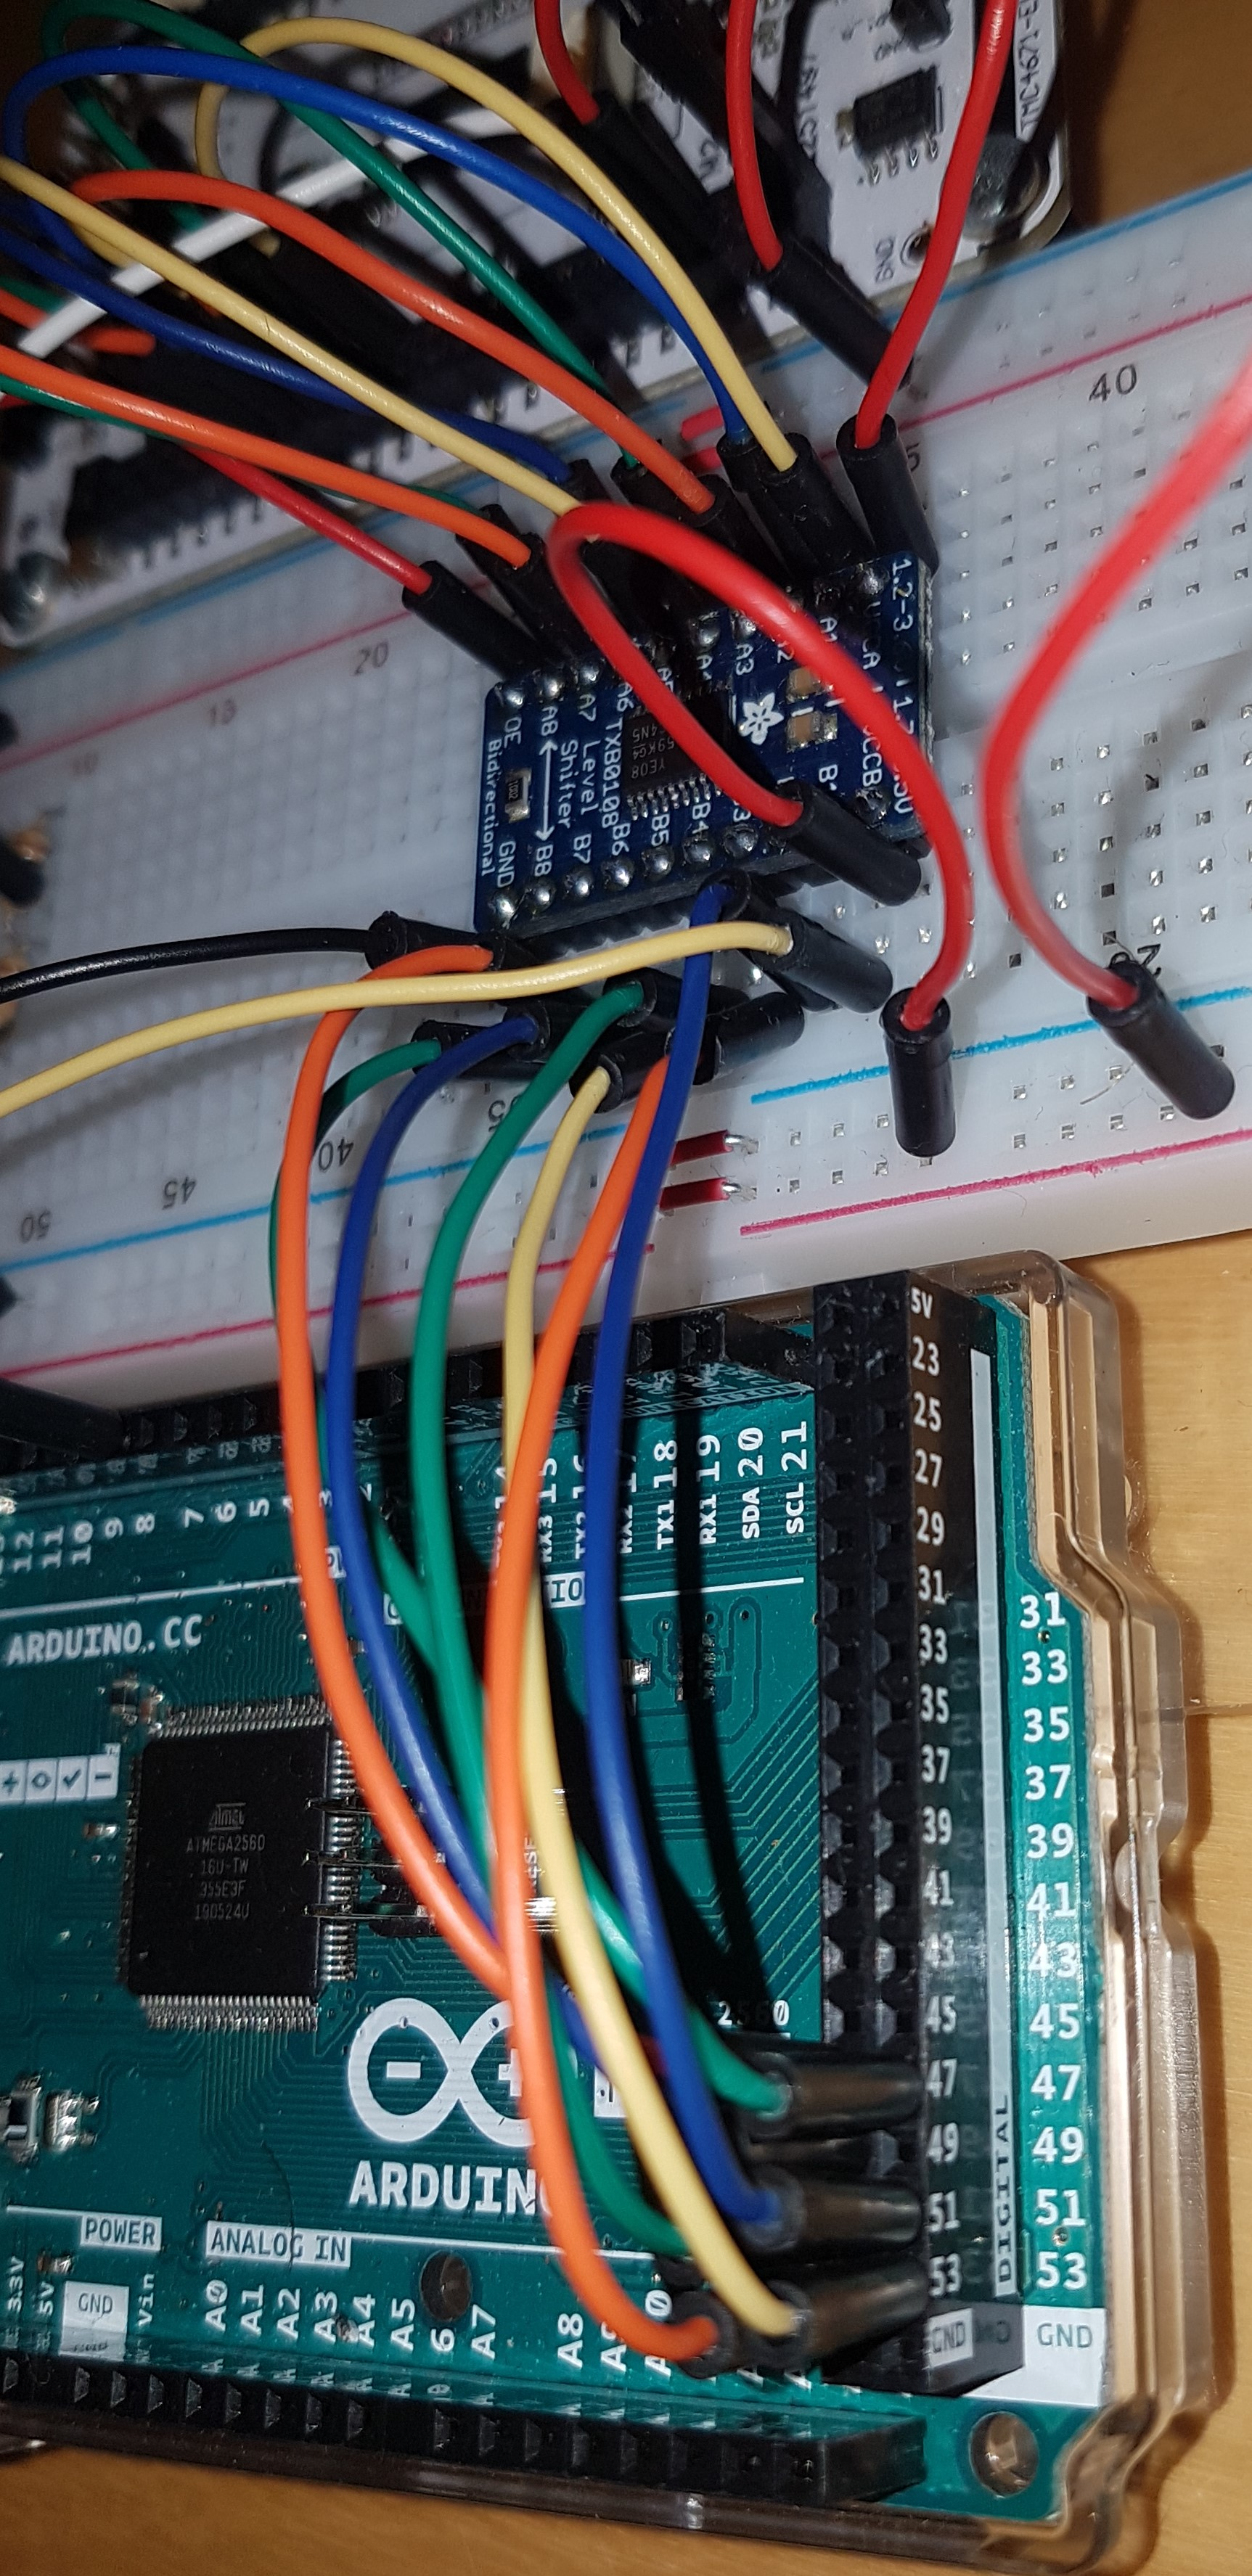
\includegraphics[angle = 270,width=\textwidth]{graphics/2_Arduino}
%	\caption{Setup mit Fokus auf Arduino.}
%	\label{fig:2_Arduino}
%\end{figure}
%
%\begin{figure}[H]
%	\centering
%	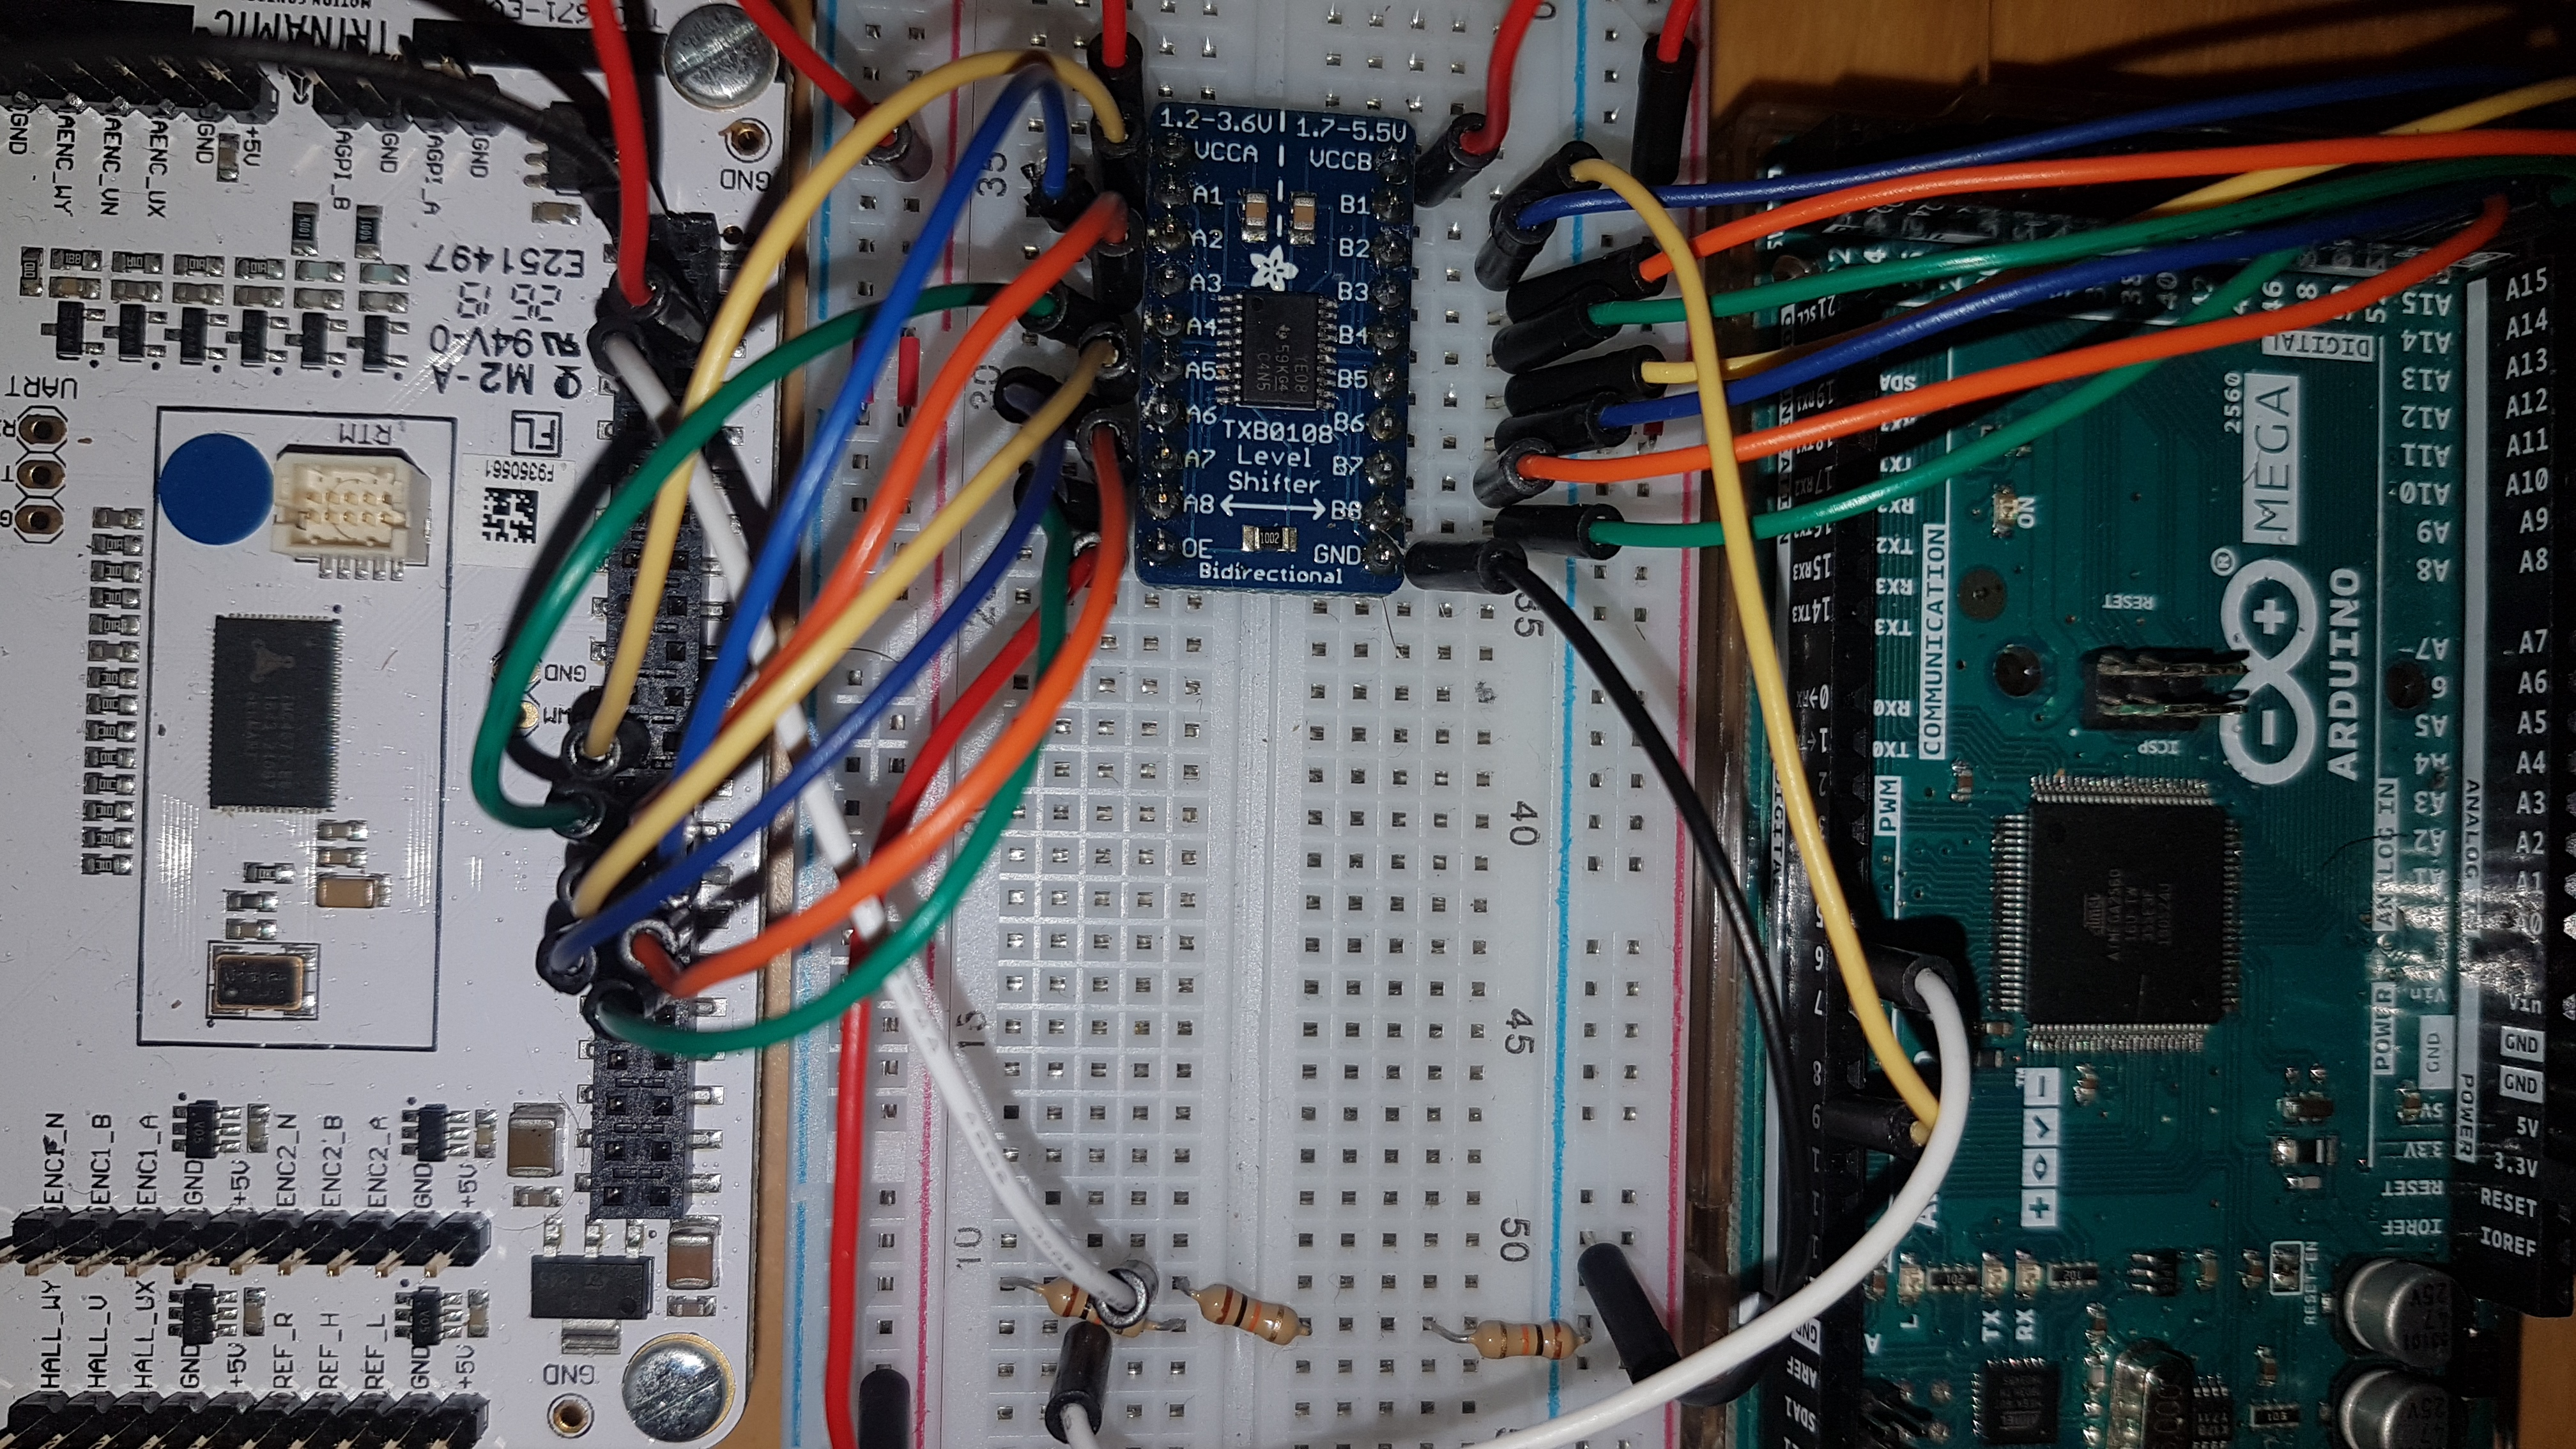
\includegraphics[angle = 180,width=\textwidth]{graphics/2_EVAL}
%	\caption{Setup mit Fokus auf TMC4674-EVAL.}
%	\label{fig:2_EVAL}
%\end{figure}
\subsection{Inbetriebnahme}

\subsubsection{Verstärkungsfaktor, Strommessung, Strommesswiderstand}\label{Appendix:Shunt}

\begin{figure}[H]
	\centering
	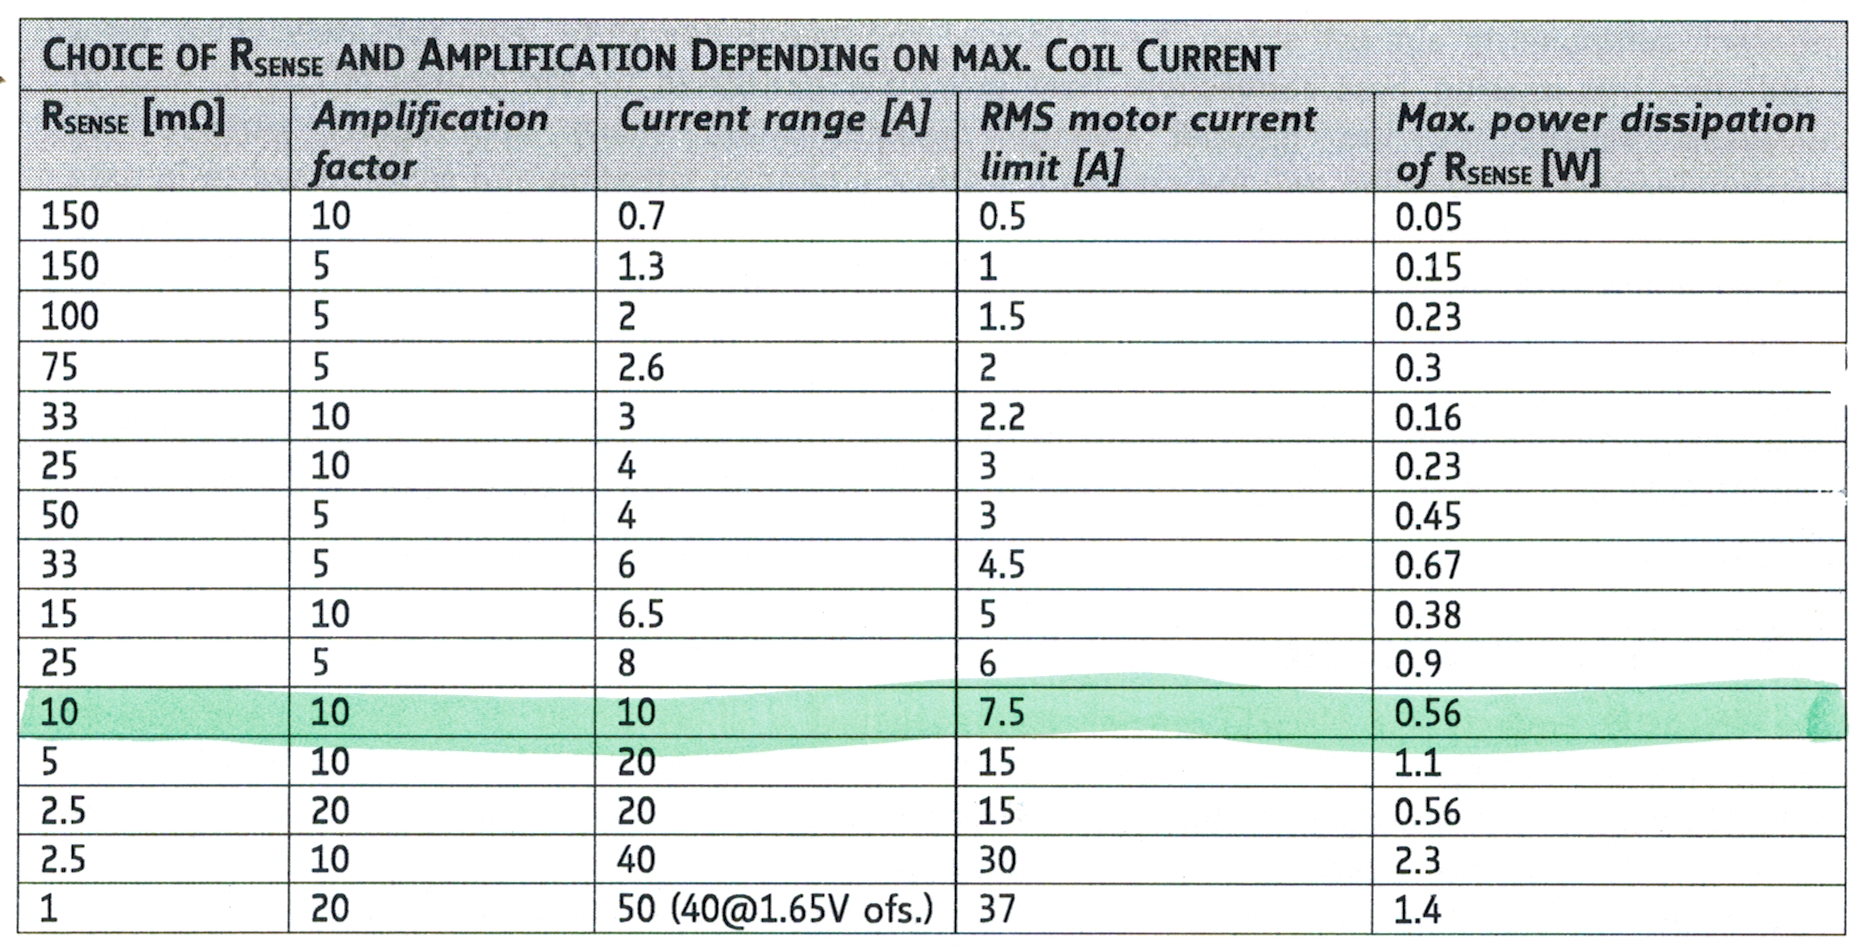
\includegraphics[width=\textwidth]{graphics/Tabelle_Shunts.png}
	\caption{Tabelle zur Bestimmung des Strommesswiderstandes aus dem Datenblatt von Trinamic.\cite[S.31]{trinamicmotion_control_gmbh__co_kg_tmc6200_2019}}
	\label{fig:Tabelle_Shunts}
\end{figure}

\subsubsection{Gate-Vorwiderstand}\label{Appendix:Gate_Vorwiderstand}

\begin{figure}[H]
	\centering
	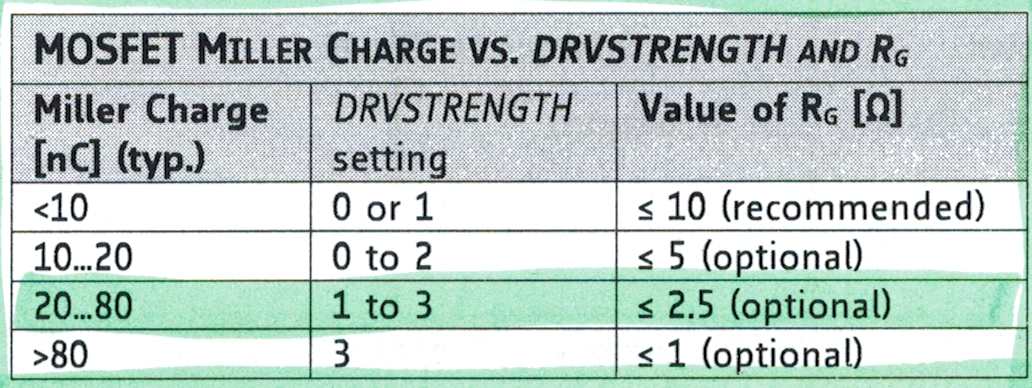
\includegraphics[width=0.5\textwidth]{graphics/Tabelle_Gatewiderstaende.png}
	\caption{Tabelle zur Bestimmung der Gatewiderstände aus dem Datenblatt von Trinamic.\cite[S.13]{trinamicmotion_control_gmbh__co_kg_tmc6200_2019}}
	\label{fig:Tabelle_Gatewiderstaende}
\end{figure}

\subsubsection{Inbetriebnahme SPI-Kommunikation}\label{Appendix:TMC6200_SPI}

%\begin{figure}[H]
%\center
%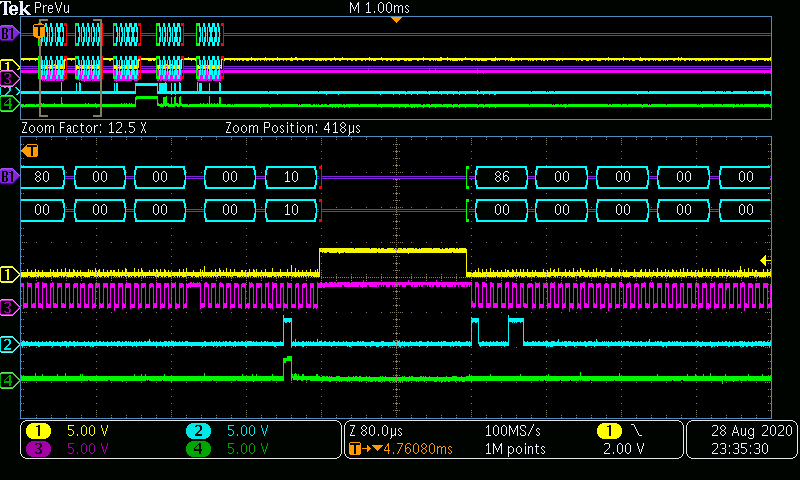
\includegraphics[width = \textwidth]{graphics/TMC6200_Beschreiben2}
%\caption{SPI-Übertragung Write 1.}
%\label{fig:TMC6200_Beschreiben2}
%\end{figure}
%
%\begin{figure}[H]
%\center
%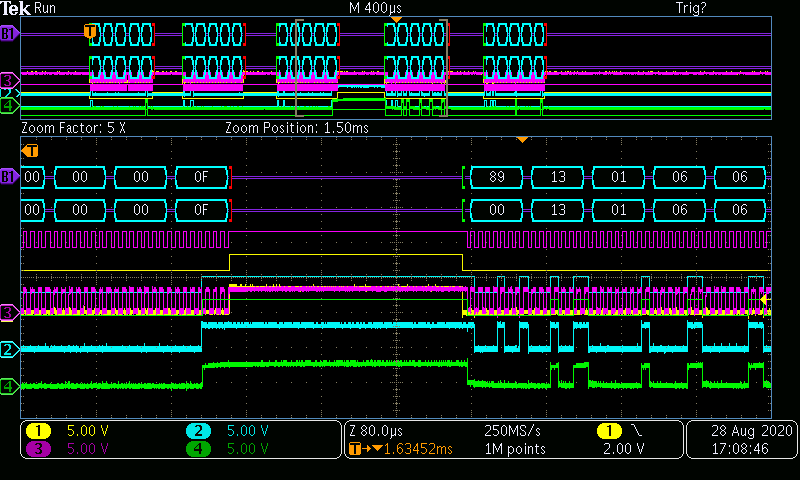
\includegraphics[width = \textwidth]{graphics/TMC6200_Beschreiben}
%\caption{SPI-Übertragung Write 2.}
%\label{fig:TMC6200_Beschreiben}
%\end{figure}

\begin{figure}[H]
\center
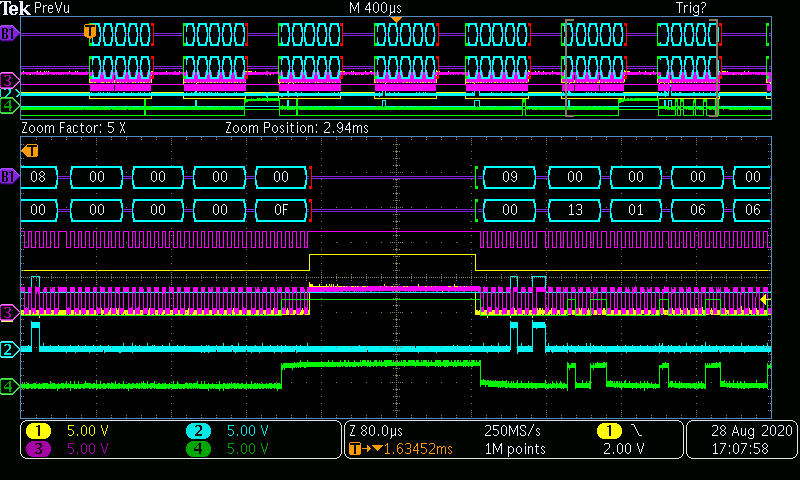
\includegraphics[width = \textwidth]{graphics/TMC6200_Lesen}
\caption{SPI-Übertragung Read.}
\label{fig:TMC6200_Lesen}
\end{figure}
%
%\begin{figure}[H]
%\center
%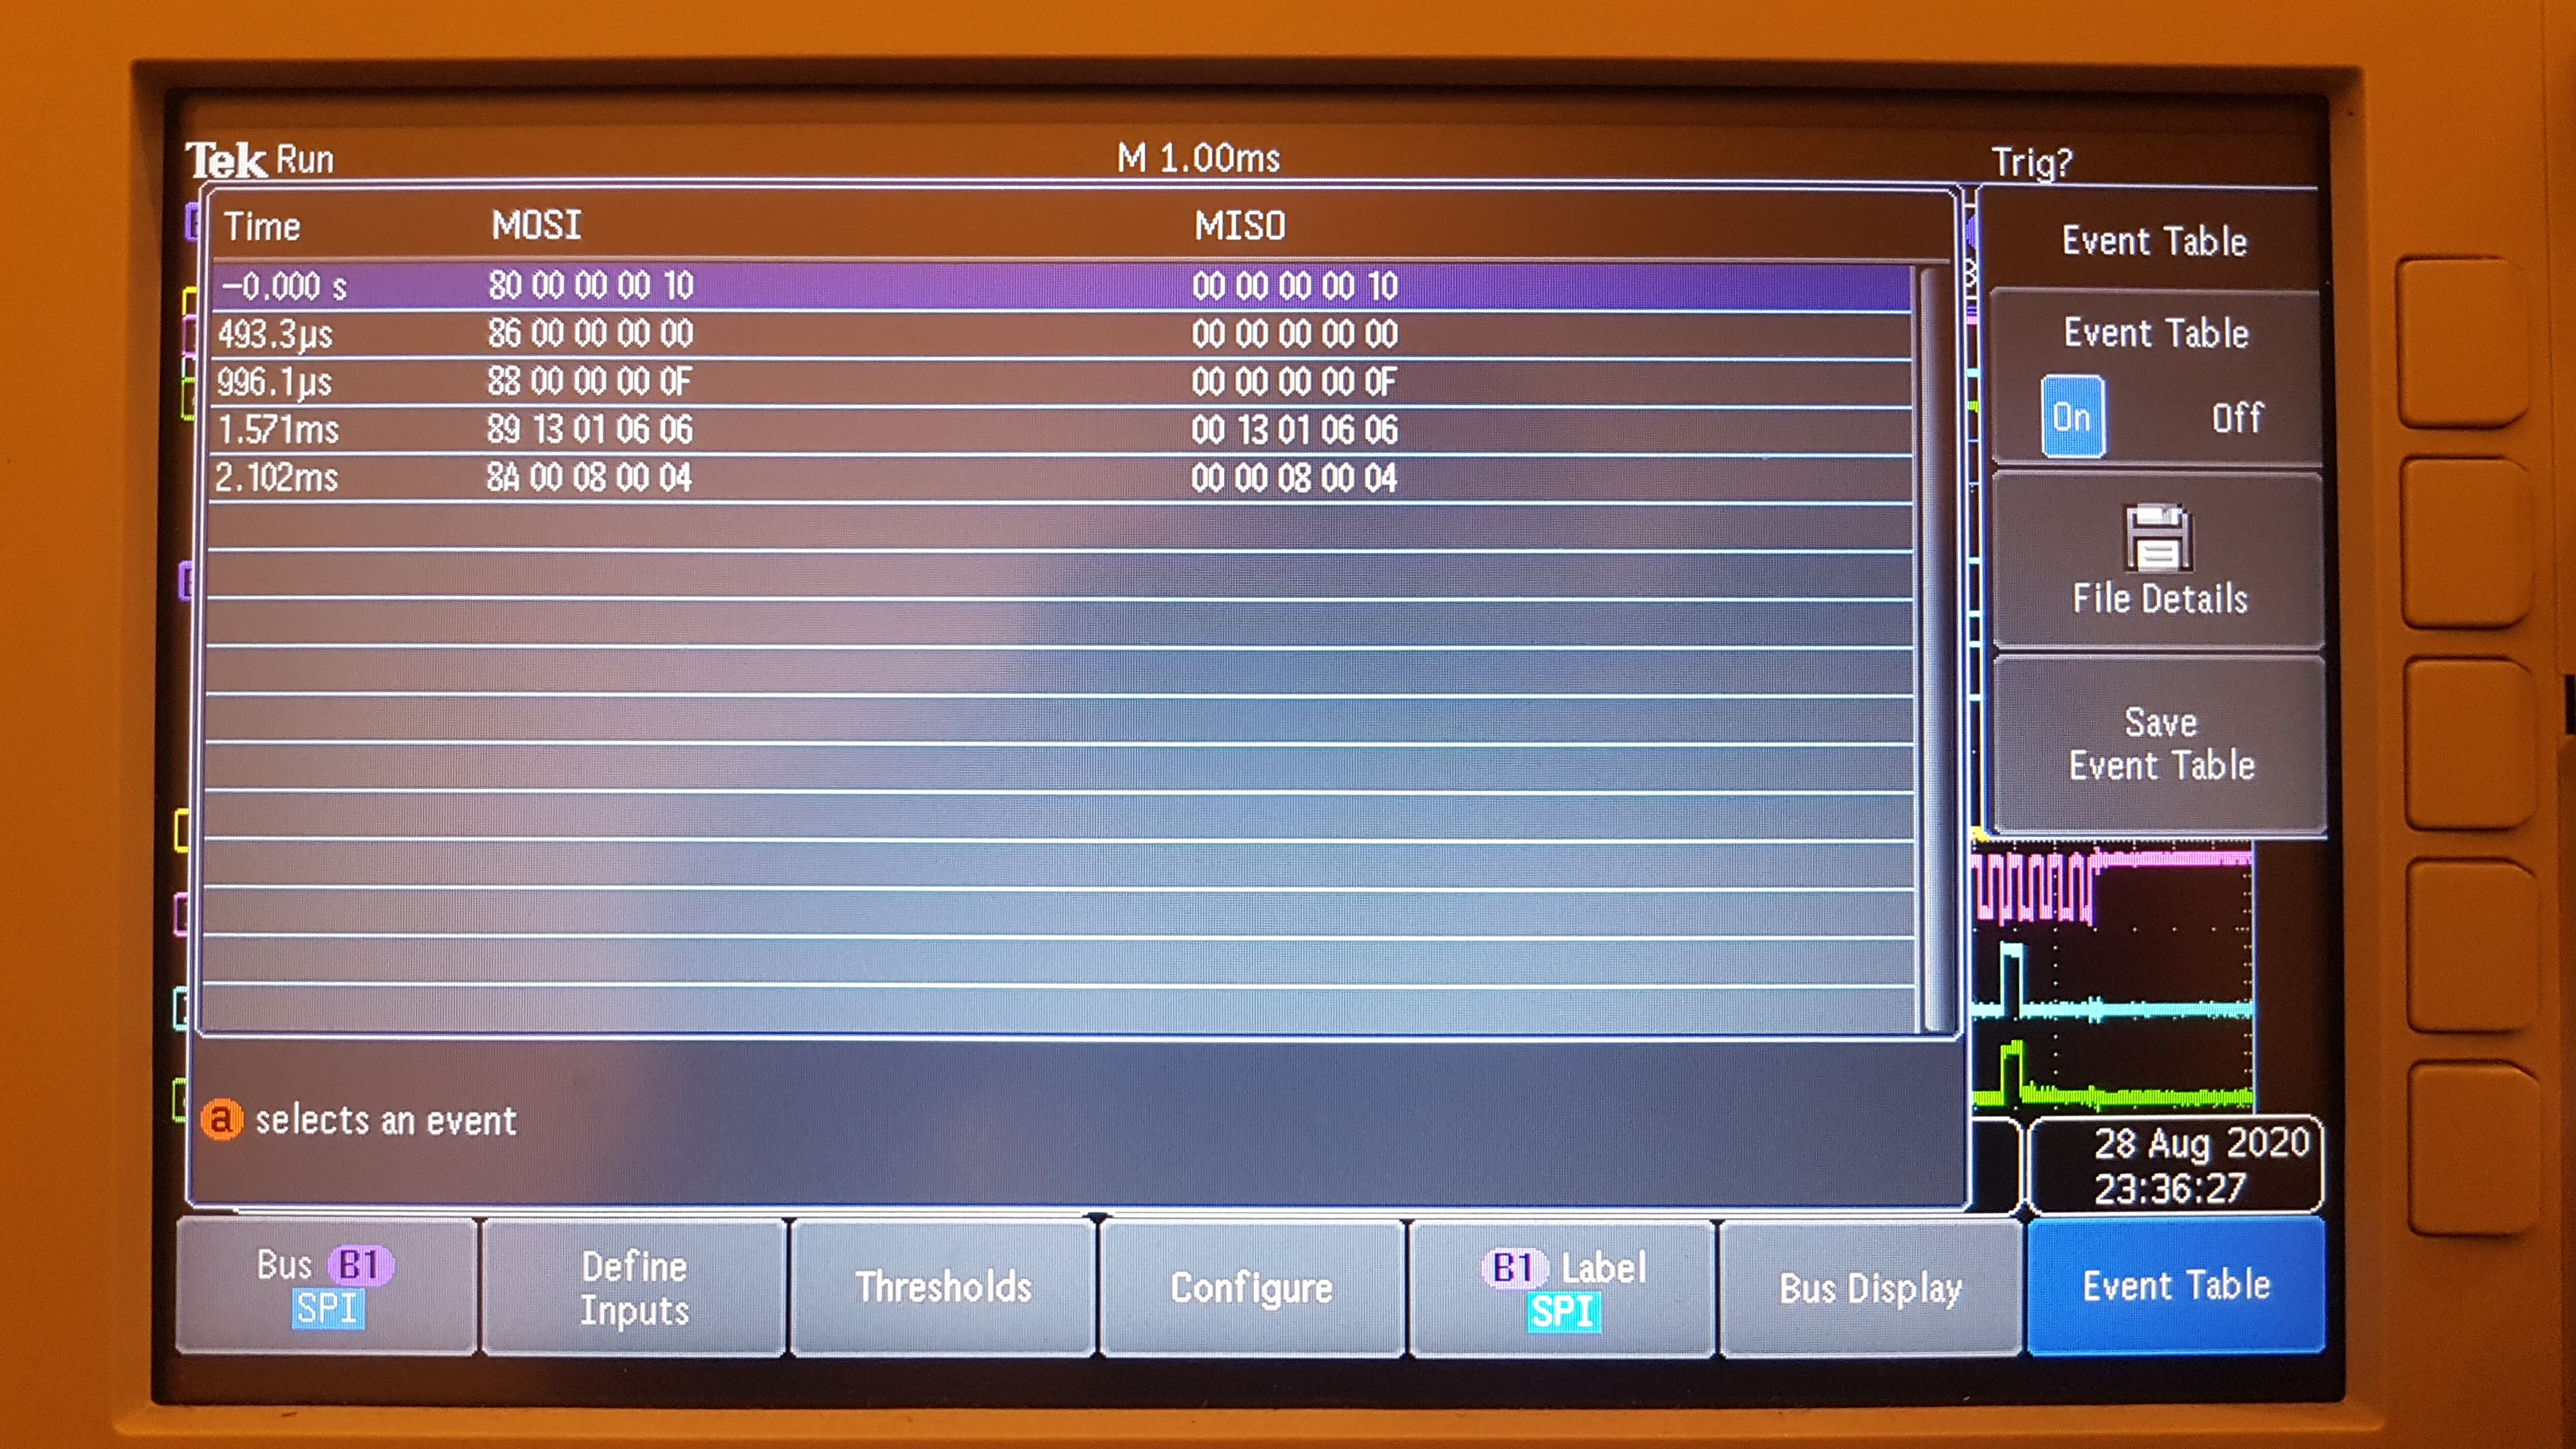
\includegraphics[width = \textwidth]{graphics/TMC6200_EventTable_Beschreiben_Bild}
%\caption{Event-Table Inbetriebnahme Gate-Treiber write.}
%\label{fig:TMC6200_EventTable_Beschreiben_Bild}
%\end{figure}

\begin{figure}[H]
\center
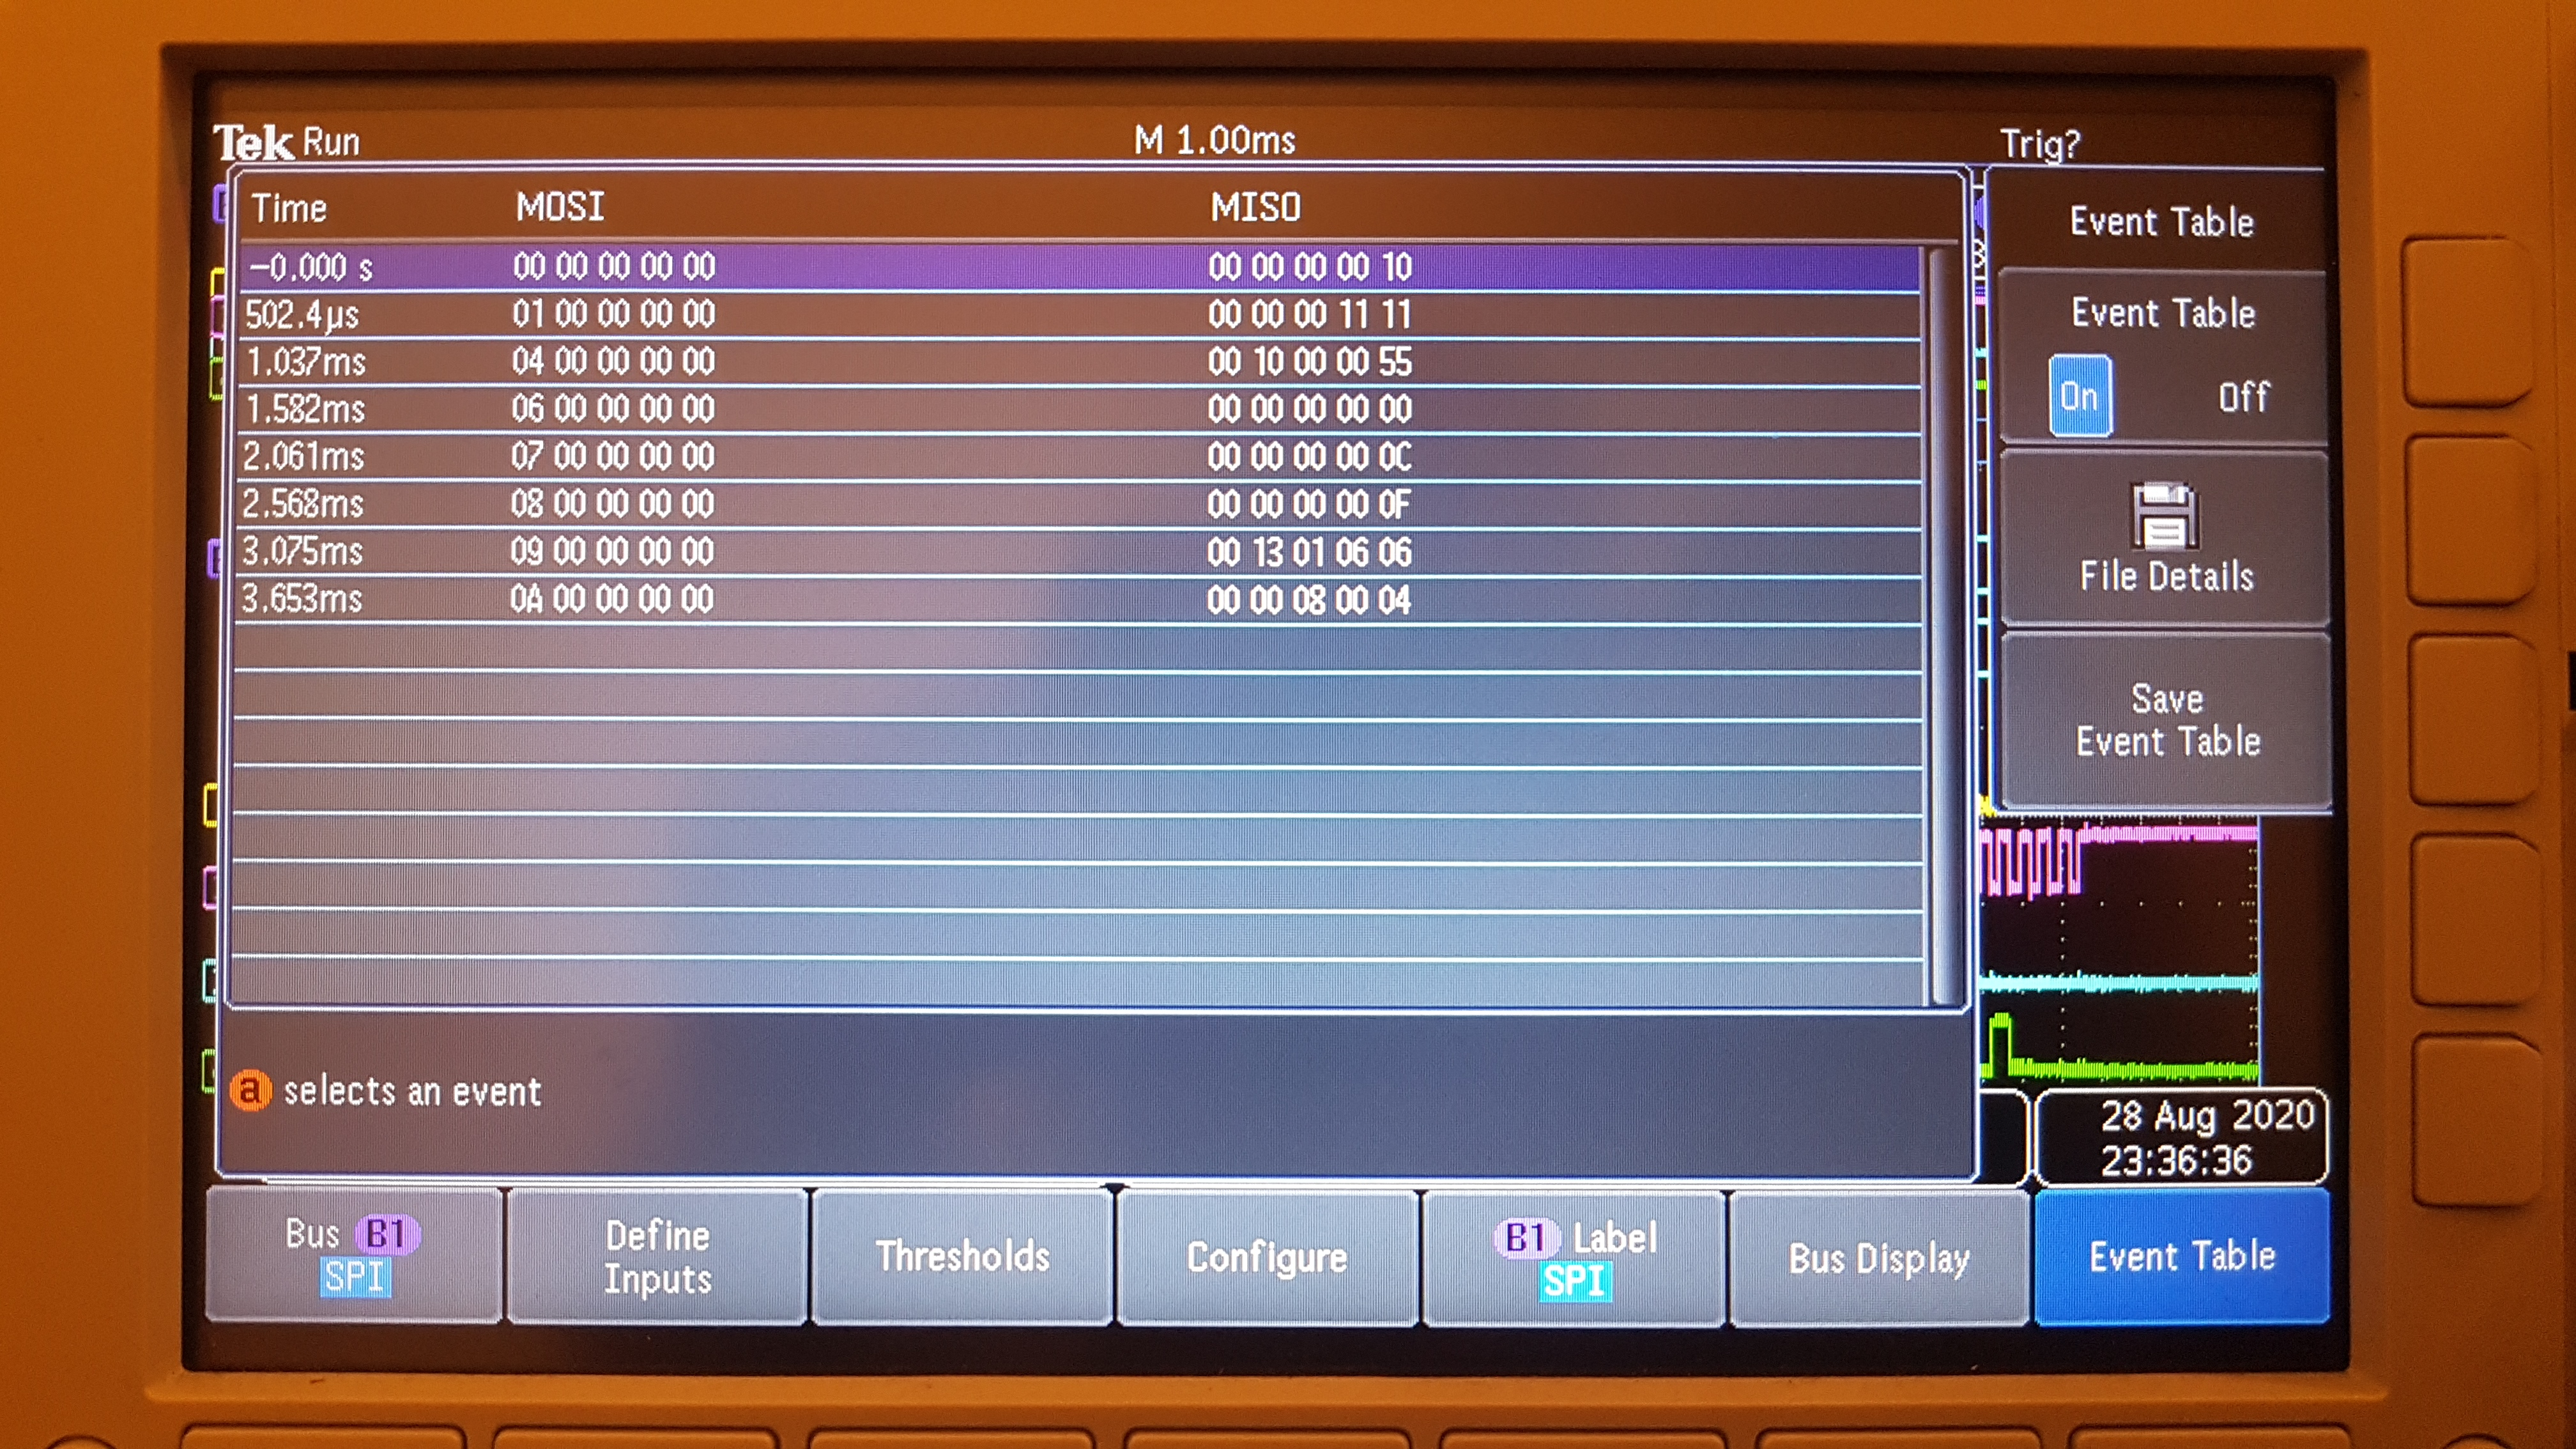
\includegraphics[width = \textwidth]{graphics/TMC6200_EventTable_Lesen_Bild}
\caption{Event-Table Inbetriebnahme Gate-Treiber read.}
\label{fig:TMC6200_EventTable_Lesen_Bild}
\end{figure}

\subsubsection{Inbetriebnahme Gate-Ctrl}\label{Appendix:TMC6200_Gate_Ctrl}

\begin{figure}[H]
\center
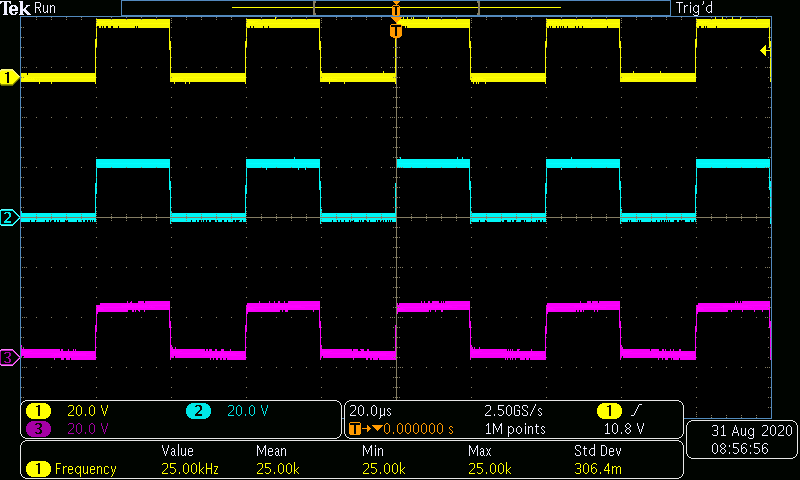
\includegraphics[width = \textwidth]{graphics/TMC6200_Gate_Signal_H}
\caption{High-Steuersignale PWM 48V von Gate-Treiber auf H-Brücke. Gelb = U, Blau = V, Magenta = W}
\label{fig:TMC6200_Gate_Signal_H}
\end{figure}

\begin{figure}[H]
\center
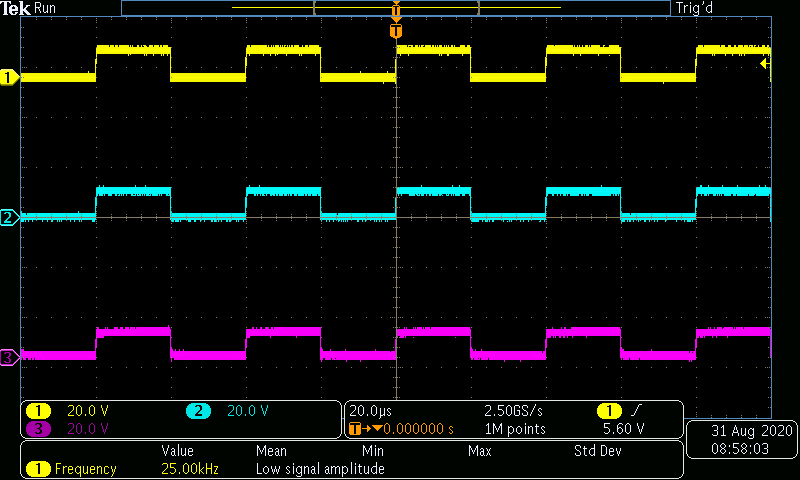
\includegraphics[width = \textwidth]{graphics/TMC6200_Gate_Signal_L}
\caption{Low-Steuersignale PWM 0V von Gate-Treiber auf H-Brücke. Gelb = U, Blau = V, Magenta = W}
\label{fig:TMC6200_Gate_Signal_L}
\end{figure}


\subsubsection{Register Gate-Treiber}\label{Appendix:TMC6200_Register}

\begin{table}[H]
\centering
\begin{tabular}{|l|l|l|l|}
\hline
\multicolumn{4}{|c|}{\textbf{Gate-Treiber Register}}          \\ \hline
\textbf{Nr.} & \textbf{Register-Name} & \textbf{Wert}       & \textbf{Was} \\ \hline
0x00         & GCONF         & 0x00000010 & Current Amplification *10    \\ \hline
0x01         & GSTAT         & 0x00000000 & Resets eventual faults from restart.    \\ \hline
0x06         & OTP\_PROG     & 0x00000000 & (TMCL-IDE)    \\ \hline
0x08         & FACTORY\_CONF & 0x0000000F & Clock Frequency (TMCL-IDE)    \\ \hline
0x09         & SHORT\_CONF   & 0x13010606 & Security settings (TMCL-IDE)    \\ \hline
0x0A         & DRV\_CONF     & 0x00080004 & Treiberstärke medium (TMCL-IDE)    \\ \hline
\end{tabular}
\end{table}
